\documentclass[12pt,a4paper]{article}
\usepackage[utf8]{inputenc}
\usepackage{graphicx}
\usepackage[margin=1.5in]{geometry}

 
\begin{document}
\begin{titlepage}
	\centering
	{\scshape\LARGE Stocks Project \par}
	\vspace{1cm}
	{\scshape\Large Design Documentation\par}
	\vspace{2cm}
	{\Large\itshape Alex Bettadapur\par}
	\vspace{1cm}
	{\Large\itshape Andy Hull\par}
	\vspace{1cm}
	{\Large\itshape Charles Wang\par}
	\vspace{1cm}
	{\Large\itshape Kendall Merritt\par}
	\vspace{1cm}
	{\Large\itshape Jason Provenzano\par}
	{\Large\itshape\par}
	\vfill
	CS 4911 Senior Design\\
Pivotal Tracker: https://www.pivotaltracker.com/n/projects/1418330
	\vfill

	{\large \today\par}
\end{titlepage}
 
\tableofcontents
 \newpage
\section{Design Alternatives}

Our requirements specify that the product we design should collect and analyze a relatively large amount of data. Our main design decisions involve where to perform the work, where and how to store the results until they are needed by the user, and how to present the results and allow the user to interact with the system. Overall, since our application is intended more as a data analysis tool, the bulk of our work will be implementing these tools and thus our design does not need to be very complex.
\vspace{.1cm}

\indent In light of these constraints, we came up with three options: Native client, Web Service, and Web Serv with Thin Client, all of which are described in more detail below. 

\subsection{Alternative 1: Native Client}

Under this alternative, we would provide the user with an application that would run on their machine. Persistent data needed by the application would be stored on the system and retrieved for analysis/presentation as necessary. The application would have a GUI to allow the user to interact with the software to change the parameters for analysis and presentation.

\subsubsection{Pros}
\begin{itemize}
\item Convenient; always accessible even without internet (even if parts of the application require internet access)
\item The user can be given the code to maintain/develop themself if desired
\item The user does not need to pay for any server/data storage services
\end{itemize}
\subsubsection{Cons}
\begin{itemize}
\item Requires space on the user's system to store data
\item Requires user's computation time to perform analysis/may tie up system resources
\item Platform dependent without any benefit for being so
\item User's system must be up while running and connected to internet constantly to perform analysis
\item User may need to run through installation hoops before being able to use the software/time required for developers to automate installation
\end{itemize}
\newpage
\subsection{Alternative 2: Web Service}

Under this alternative, we would provide a web service run on a server that would host a webpage where the user could interact with the software. This has the benefit of externalizing all the services so the user's own system is not needed for any part of the software. 

\subsubsection{Pros}
\begin{itemize}
\item Does not consume user's resources (space or computation time)
\item Platform independent
\item Can run completely independently of the user's system
\item No installation required on the user's end
\end{itemize}
\subsubsection{Cons}
\begin{itemize}
\item User may need to pay for external services
\item Internet access required to interact with application
\end{itemize}

\subsection{Alternative 3: Web Server with Thin Client}

Under this alternative, we would provide the user with a lightweight client backed by a server. The data would be stored on the server and any computations would be performed on the server. The user would interact with the application via a small UI on their system.

\subsubsection{Pros}
\begin{itemize}
\item Consumes few of user's own system resources
\item Allows for minor tasks to be migrated to user's system so no internet access required for small tasks
\end{itemize}
\subsubsection{Cons}
\begin{itemize}
\item User may need to pay for external services
\item Internet access required for important tasks
\item Platform Dependent for UI development
\item Some installation required for the user to use any tools
\item Need to develop a thin client independent of the server
\end{itemize}
\newpage
\section{Final Design and Rationale}

Based on the user's requirements and limitations, we decided to implement the project as a web service. This provides the most freedom to the user  by not tying them to any particular platform and not requiring the user's resources  to run the application.  Furthermore, the user does not need to install any packages or libraries in order to use the application. These considerations helped us to eliminate the native client alternative. 
\vspace{.1cm}

\indent The thin client alternative was very similar to the web service alternative. However, we decided to use a web service because there were not enough functions the user requested that could be reasonably moved to the user's system without making the client very heavy or causing it to consume too many resources. Furthermore, for this small benefit (some small tasks which the user only requested as auxiliary functionality), the user would need to go through some installation hassle in order to set up the thin client. At this point, the only purpose of the client would be to interact with the server. Since this is the case, internet access would always be required to do anything important and we think that the extra development cost to implement a user-side client that would only interact with a server would be wasted.

\subsection{Static Design}

Our application has three main components: a python service, web scraping tools/UI, and a database. This is detailed in figure 1 below.

\begin{figure}[h!]
  \centering
  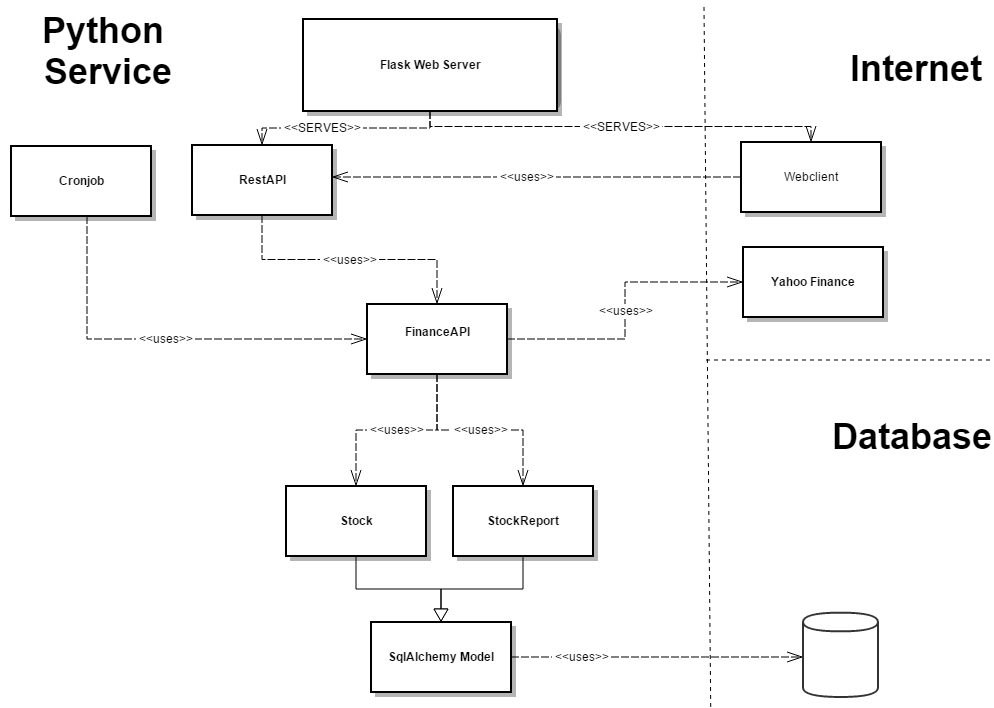
\includegraphics[scale=0.4]{stock_uml.png}
  \caption{static design}
\end{figure}

\subsection{Dynamic Design}

Our application has two main functions. One scenario corresponds to the user's requirements for stock tracking and analysis. This function uses the settings from the UI to collect and analyze stock data that are then submitted to the user in the form of a weekly (or however often the user wants) report. 
\vspace{.1cm}

\indent The second scenario consists of tools which do not contribute to the scheduled report, but may provide useful information to the client. These tools are provided to track extra information about stocks, filter stocks by some threshold, or search social media for keywords related to the stocks. The user will interact with these via the webpage. This function responds to requests the user makes through the tools page of the UI. 
\vspace{.1cm}

\indent Thus, we will have three main components: the UI, server, and database. In first scenario, the server will use the settings from the UI settings page to obtain and analyze data gathered from the Yahoo Finance public API. The server will then put this data into the database until it is needed for report generation. When the scheduled report generation takes place, the server will gather the data from the database, format it appropriately (see figure 4 in the Data section), create a pdf, and send the report via email to the client.

In a typical use case in the second scenario, the user will interact with the requested tools via the UI. The server will respond to the request, gather data from either the Yahoo Finance API or social media APIs, and then analyze the data and display results or put information in the database as appropriate. 

\begin{figure}[h!]
  \centering
  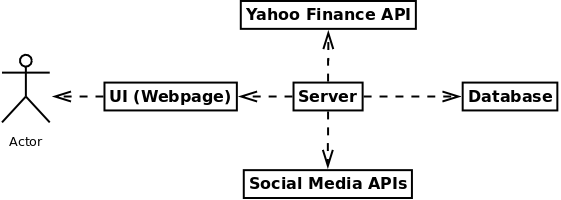
\includegraphics[scale=0.4]{UML_block.png}
  \caption{simple block diagram showing the sytem's dynamic view}
\end{figure}

Essentially, the dynamic behavior of our application is that the user will interact with the UI (webpage) to request some service. The server will then fulfill this request by gathering the relevant data and reporting the results as appropriate (for example, either delivering a schedule report, or changing the state of a display on the  UI).

\section{Data}

\subsection{Database}

Currently, our database is very simple because we have only implemented the basic requirements. It consists of a single entity with four attributes and no relations. We considered using a different format (CSV, etc.) to improve performance, but we decided that having a database would be better because we could easily grow the amount of data we keep track of in a principled way as we continue to work on the project. Stock symbol is the identifier for the stock. Float is the volume of tradeable shares available. Growth is the percentage growth of the stock over a period of time. Movement is how much the price has changed in a period of time.

\begin{figure}[h!]
  \centering
  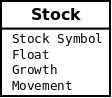
\includegraphics[scale=0.5]{simple_ER.png}
  \caption{simple ER diagram fulfilling client's basic requirements}
\end{figure}

For example, one extra feature the client has requested is the ability to search for keywords related to stocks on social media. For exapmle, the words ``Merger", ``Buyout", ``Takeout", and ``Acquisition" could all indicate something important that the client would want to know about when trading stocks. Thus, we could associate keywords with stocks in the database as follows:
\\
\begin{figure}[h!]
  \centering
      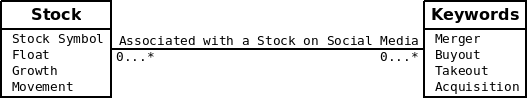
\includegraphics[scale=0.7]{More_ER.png}
  \caption{slightly more complicated ER diagram}
\end{figure}

Currently, we do not have any more complex requirements from the client, but it's easy to see how this could be complicated by the addition of a lot of extra features which are relevant to stock trading. Furthermore, we can use a database easily because we do not need to write our own code to parse our own data storage files. Thus, we decided to use a database to allow for easy addition of complexity to the application as well as ease of implementation.

\subsection{Report}

The client requested the periodic delivery of a report that lists all the stocks that meet their requirements. To do this, we decided to use HTML to format with a table containing the filtered stocks and their relevant attributes in a table in the following format:

\begin{figure}[h!]
\centering
    \begin{tabular}{ | l | l | l | l | l | l |}
    \hline
    Stock Symbol & Float & Growth & Movement & Attribute & ... \\ \hline
    AAPL & 5.70B & 32.50\% & +23.50\% & Value & ...\\ \hline
    MSFT & 7.36B & -5.10\% & -15.00\% & Value & ... \\ \hline
    ... & ... & ... & ... & ... & ...\\ \hline
    \end{tabular}
\caption{Stock Report format}
\end{figure}

We selected this format, and not something like a CSV or other more analysis friendly format because the nature of the data makes it unsuitable for any particular analysis or graphing. In particular, the data is only reported when it is above the client's specified thresholds, so only the value is important. Furthermore, we have included graphing utilities in the web service so that the client will not need to perform these operations manually.

\section{Detailed Design}

Since our application is not object oriented, we do not need a very complicated analysis. Therefore, most of the following discussion will refer to the figures already presented. 

\subsection{Static Design}
	
Figure 1 shows the structure of our application and the relationship between the components. Descriptions of each component are given below.
\begin{itemize}
\item webserver: This component knows how to process and fulfill requests from the web client 
\item cronjob: This component holds information about when to generate the scheduled reports
\item restAPI: This component details how to interact with the webclient
\item financeAPI: This component details how to fulfill requests by analyzing the data
\item yahoo finance API: This component provides stock information necessary to process the user's requests
\item webclient: This component provides a UI for the user to interact with the web server through a layer of abstraction
\item stock: This component models the stock object for the system to provide a uniform data retrieval/storage for stocks
\item stockreport: This component holds the directions for creating the stock reports that the user requested
\item sqlalchemy: This component converts stock information into database entires
\item database: This component stores all the persistent information we need about stocks to perform the user's jobs
\end{itemize}

\subsection{Dynamic Design}

\begin{itemize}
\item webclient: The user initiates requests on the webclient and inputs the settings they want for their analysis. 
\item webserver: The webserver receives information about the user's desired settings and requests and proceeds to fulfill the user's requirements using various APIs
\item rest API: The server uses the rest API to interact with the web client and other APIs
\item financeAPI: The server uses the financeAPI to gather information about stocks and then provide analysis corresponding to the user's requirements
\item yahoo finance API: The financeAPI uses the Yahoo Finance API to scrape information about stocks for processing
\item stock: The finance API stores information about stocks a Stock
\item stockreport: The finance API directs stock report generation as scheduled by the cronjob
\item cronjob: The cronjob tells the financeAPI when to generate stock reports
\item sqlalchemy: sqlalchemy converts the stock and stockreport information into database entires
\item database: The database stores persistent stock information needed for analysis and report generation
\end{itemize}

\section{UI}

The main method of interaction with the application will be through a webpage. Preliminary mockups of the webpage have been provided below. The webpage displays by default a home screen. The user can then navigate, using a navigation bar to settings and tools pages. The settings page allows the user to modify the parameters for data analysis and the tools page contains extra functionality the user requested independent of the weekly report.
\vspace{0.1cm}

\indent Since the user did not explicitly request a webpage, we do not have any requirements that need to be met with respect to the user interface. However, we plan to make the UI a webpage because we believe this is the best way to allow the user to interact with the application. The user will navigate through the pages using tabs (seen in the upper right hand corner). On the homepage, we plan to have some passive graphics related to data generated by the user's requests. 

\begin{figure}[h!]
  \centering
  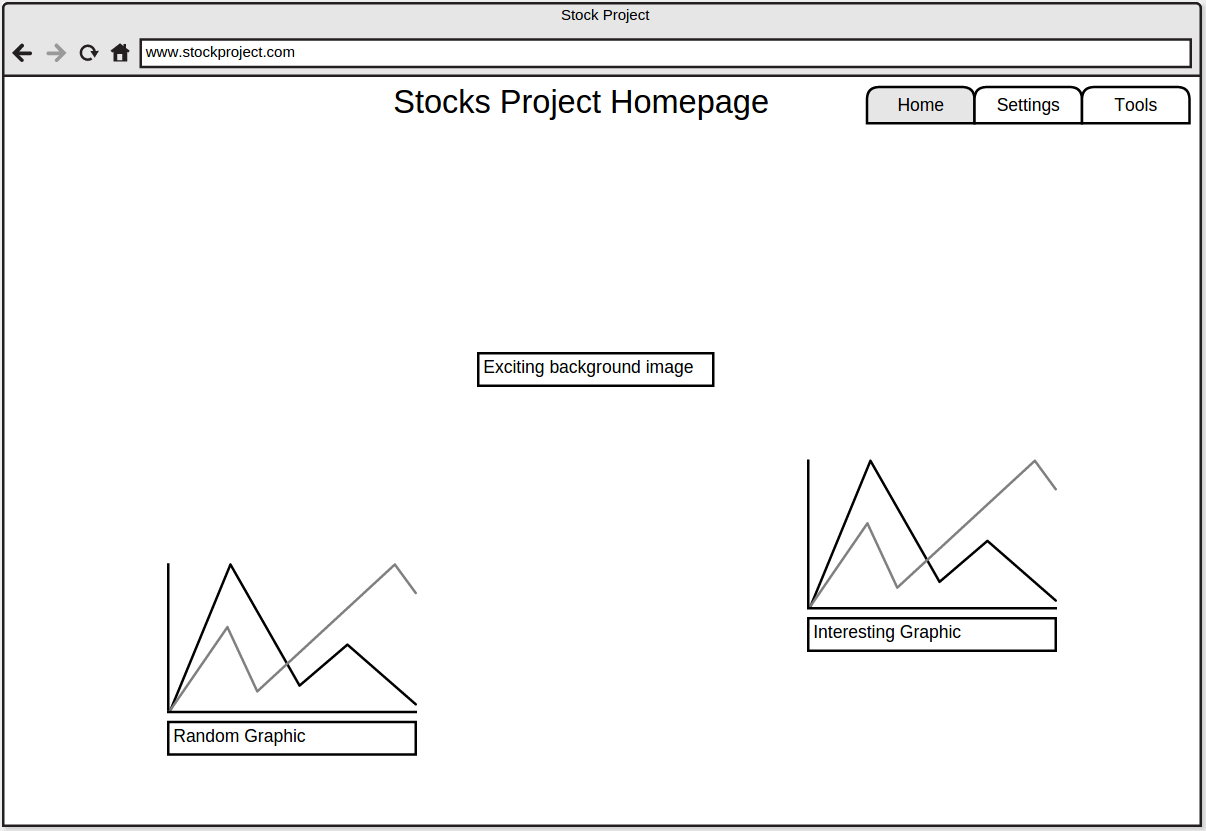
\includegraphics[scale=0.3]{homepage.png}
  \caption{Simple home page mockup}
\end{figure}

On the settings page, the user will enter their email address (in order to receive reports) as well as the desired thresholds/attributes for the data analysis. Here, the user will also be able to decide how often to receive reports and any other settings that the user communicates to us in the future. See figure 7 (next page) for a sample mockup of the settings page.

\begin{figure}[h!]
  \centering
  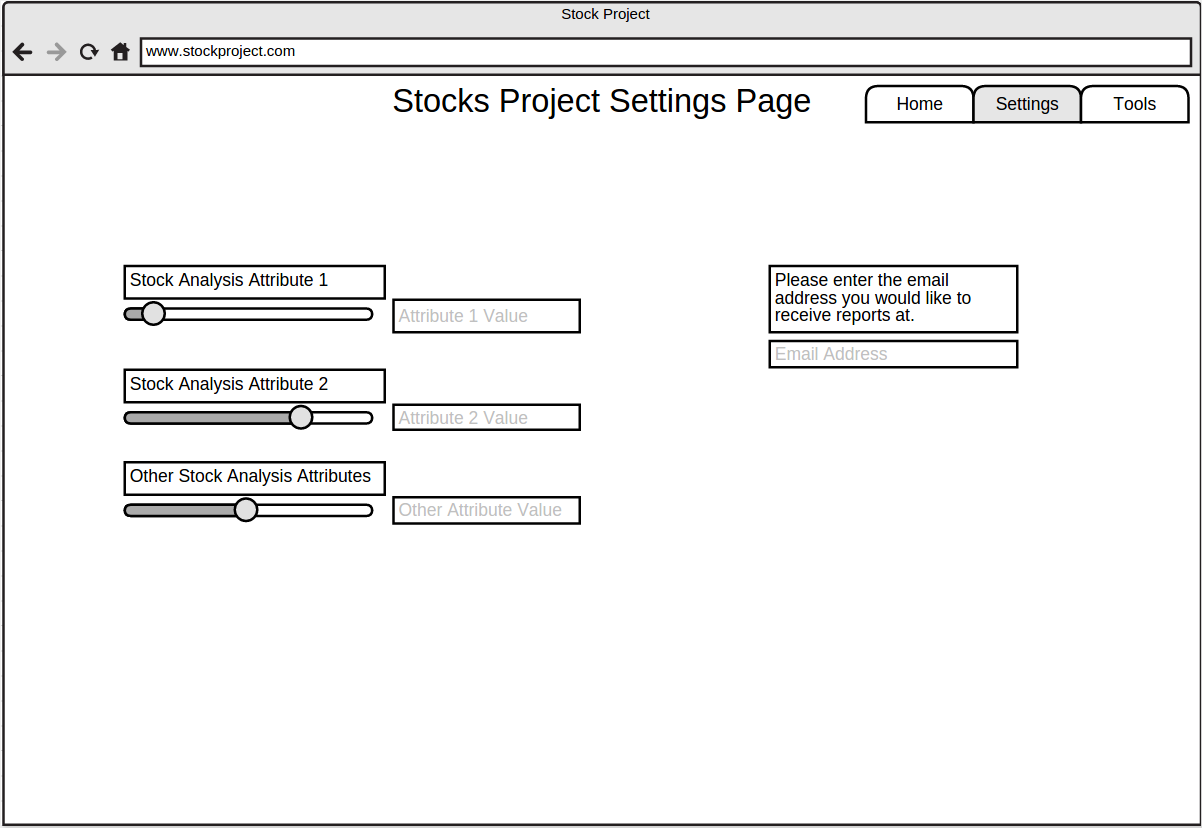
\includegraphics[scale=0.3]{settingspage.png}
  \caption{Simple settings page mockup}
\end{figure}

Finally, the tools page will contain extra tools (not related to the periodic report). For example, the user could obtain information about individual stocks, search social media for keywords, etc.

\begin{figure}[h!]
  \centering
  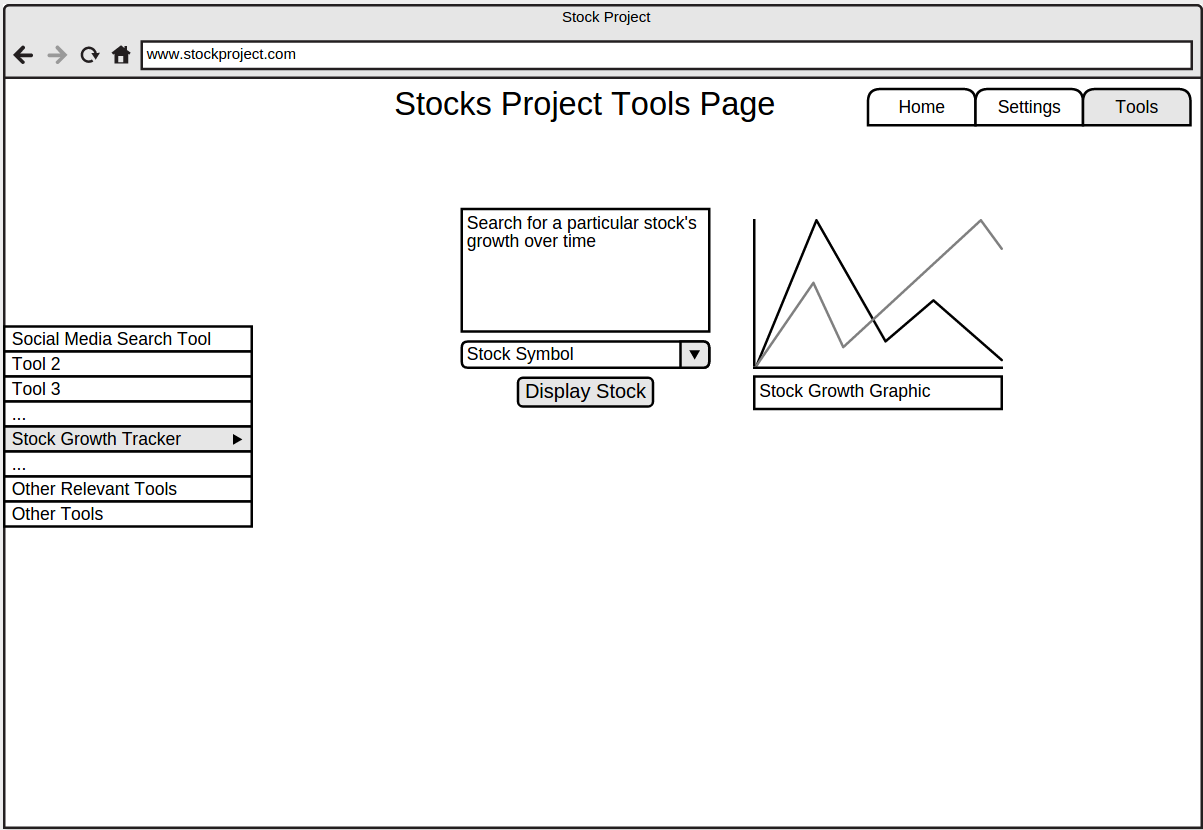
\includegraphics[scale=0.3]{toolspage.png}
  \caption{Simple tools page mockup}
\end{figure}

\section{Validation}
 
\begin{enumerate}
\item User Story: As a user, I want to receive scheduled emails containing information about stocks fitting my requirements. 
\begin{enumerate}
\item Requirements:
\begin{enumerate}
\item Scheduling: We will use a cronjob to schedule periodic (weekly) reports
\item Find Stocks: We will use the FinanceAPI to calculate metrics about the stocks and compare them to the user's threshold values 
\item Report Generation: We will use StockReport to create reports from stocks meeting the threshold requirements
\item Email: The server will send an email with the generated report attached
\end{enumerate}
\item Status: Pass.  We have components to perform each task necessary to fulfill this user story.
\end{enumerate}
\item User Story: As a user, I want to be able to modify the attribute thresholds for reporting stocks 
\begin{enumerate}
\item Requirements:
\begin{enumerate}
\item UI: The webclient will serve as the UI through which the user can modify the attributes
\item attribute thresholds: The server will store the threshold data which will be used for reporting stocks
\end{enumerate}
\item Status: Pass. We have components to perform each task necessary to fulfill this user story.
\end{enumerate}
The user has also requested more tools, but we do not have the explicit details of how these tools should work. Some sample user stories of these tools are provided below:
\item User Story: As a user, I want to be able to search social media for keywords about stocks
\begin{enumerate}
\item Requirements:
\begin{enumerate}
\item Search social media: We will need to integrate some social media APIs  (twitter, for example) to search for keywords
\item UI: We will need to add functionality to the UI to do this
\item Server: server should display the relevant stock information for any keywords found in the context of a stock (for example, if a stock's twitter feed had important words such as merger, buyout, etc.)
\end{enumerate}
\item Status: No Pass. We will add this functionality when the details are made  explicit.
\end{enumerate}
\item User Story: As a user, I want to be able to see the metrics for individual stocks, even if they are not featured in the report
\begin{enumerate}
\item Requirements:
\begin{enumerate}
\item Display stock information: We will need to add this functionality to the UI
\item FinanceAPI: retrieve stock information using Yahoo Finance API and process data to provide metrics
\end{enumerate}
\item Status: No Pass. We will add this functionality when the details are made explicit. However,  most of the infrastructure to do this is already in place so this should be relatively easy to implement quickly.
\end{enumerate}
\end{enumerate}

We have essentially finished the core part of the application that the client initally requested. We will continue add tools the client wants to develop this project according to the client's needs and we will make sure to stay up to date with the client's evolving requirements. 

\end{document}


CS4911 Design Documentation
Architecture and Rationale

It should give
a representation of how your application will interact with external
entities and how it is organized. 
It is important to provide both a static and dynamic view of your
architecture. A static view might, for example, be expressed with a UML
Package diagram. A dynamic view could be a system-level sequence
diagram or a textual description of how functionality is realized at the
architectural level. Each component should be indentified as to what 
functionality it provides and how it interoperates with other components
to form a working system. The dynamic description can be a textual
walkthrough of the architecture along with a scenario, or it can be a
sequence diagram.

Detailed Design
Decompose the high-level architecture into the lower level classes and
document their dynamic behavior. If a non-OO application, document
the static and dynamic behavior of the application. Typically, for UML
this would be a class diagram and any of: state diagram, sequence
diagram, collaboration diagram, or activity diagram.
For web applications, this might include a page navigation graph, along
with summaries of the scripts running on each page.
GUI
Many modern systems are interactive. That is, the user interacts with
the system using some form of display screen using which data can be
entered and results presented. Well-designed GUIs are essential to
successful systems because they are the most visible part of the
system. As such, it is important to get early and frequent feedback from
users about their reactions. This can take the form of a prototype, but if
this is infeasible, then mocked up screen shots can be substituted. Your
design documentation should include a description of your user
interface design. You should explain what the viewer is looking at for
each screen. Even command line apps have a UI and you should
describe the command line options. If you are making a library rather
than an application, then explain your API.
Validation
Every stage of software development should be validated. This is
particularly true of design, because design is the most accessible
description of the problem's solution. There are a variety of ways to
validate software designs, but all of them involve comparing the design
with the user needs. Examples include requirements tracing, nonfunctional
requirements walkthroughs, or scenario-based evaluation
methods. You should document the steps that you will take to validate
your design. You may include the results here or in your individual
design assessment.